%package list
\documentclass{article}
\usepackage[top=3cm, bottom=3cm, outer=3cm, inner=3cm]{geometry}
\usepackage{multicol}
\usepackage{listings}
\usepackage[utf8]{inputenc}
\usepackage{graphicx}
\usepackage{url}
%\usepackage{cite}
\usepackage{hyperref}
\usepackage{array}
%\usepackage{multicol}
\newcolumntype{x}[1]{>{\centering\arraybackslash\hspace{0pt}}p{#1}}
\usepackage{natbib} 
\usepackage{pdfpages}
\usepackage{multirow}   
\usepackage[normalem]{ulem}
\useunder{\uline}{\ul}{}
\usepackage{svg}
\usepackage{xcolor}
\usepackage{listings}
\lstdefinestyle{ascii-tree}{
    literate={├}{|}1 {─}{--}1 {└}{+}1 
  }
\lstset{basicstyle=\ttfamily,
  showstringspaces=false,
  commentstyle=\color{red},
  keywordstyle=\color{blue}
}
%\usepackage{booktabs}
\usepackage{caption}
\usepackage{subcaption}
\usepackage{float}
\usepackage{array}

\newcolumntype{M}[1]{>{\centering\arraybackslash}m{#1}}
\newcolumntype{N}{@{}m{0pt}@{}}


%%%%%%%%%%%%%%%%%%%%%%%%%%%%%%%%%%%%%%%%%%%%%%%%%%%%%%%%%%%%%%%%%%%%%%%%%%%%
%%%%%%%%%%%%%%%%%%%%%%%%%%%%%%%%%%%%%%%%%%%%%%%%%%%%%%%%%%%%%%%%%%%%%%%%%%%%
\newcommand{\itemEmail}{ shanccom@unsa.edu.pe }
\newcommand{\itemStudent}{ Sergio Hancco Mullisaca }
\newcommand{\itemCourse}{Programacion Web 2}
\newcommand{\itemCourseCode}{}
\newcommand{\itemSemester}{II}
\newcommand{\itemUniversity}{Universidad Nacional de San Agustín de Arequipa}
\newcommand{\itemFaculty}{Facultad de Ingeniería de Producción y Servicios}
\newcommand{\itemDepartment}{Departamento Académico de Ingeniería de Sistemas e Informática}
\newcommand{\itemSchool}{Escuela Profesional de Ingeniería de Sistemas}
\newcommand{\itemAcademic}{2024 - A}
\newcommand{\itemInput}{Del 8 Mayo 2024}
\newcommand{\itemOutput}{Al 15 Mayo 2024}
\newcommand{\itemPracticeNumber}{3}
\newcommand{\itemTheme}{JAVASCRIPT}
%%%%%%%%%%%%%%%%%%%%%%%%%%%%%%%%%%%%%%%%%%%%%%%%%%%%%%%%%%%%%%%%%%%%%%%%%%%%
%%%%%%%%%%%%%%%%%%%%%%%%%%%%%%%%%%%%%%%%%%%%%%%%%%%%%%%%%%%%%%%%%%%%%%%%%%%%

\usepackage[english,spanish]{babel}
\usepackage[utf8]{inputenc}
\AtBeginDocument{\selectlanguage{spanish}}
\renewcommand{\figurename}{Figura}
\renewcommand{\refname}{Referencias}
\renewcommand{\tablename}{Tabla} %esto no funciona cuando se usa babel
\AtBeginDocument{%
	\renewcommand\tablename{Tabla}
}

\usepackage{fancyhdr}
\pagestyle{fancy}
\fancyhf{}
\setlength{\headheight}{30pt}
\renewcommand{\headrulewidth}{1pt}
\renewcommand{\footrulewidth}{1pt}
\fancyhead[L]{\raisebox{-0.2\height}{\includegraphics[width=3cm]{logo_episunsa.png}}}
\begin{figure}
    \centering
    \label{fig:enter-label}
\end{figure}
\fancyhead[C]{\fontsize{7}{7}\selectfont	\itemUniversity \\ \itemFaculty \\ \itemDepartment \\ \itemSchool \\ \textbf{\itemCourse}}
\fancyhead[R]{\raisebox{-0.2\height}{\includegraphics[width=1.2cm]{}}}
\fancyfoot[C]{\itemCourse}
\fancyfoot[R]{Página \thepage}

% para el codigo fuente
\usepackage{listings}
\usepackage{color, colortbl}
\definecolor{dkgreen}{rgb}{0,0.6,0}
\definecolor{gray}{rgb}{0.5,0.5,0.5}
\definecolor{mauve}{rgb}{0.58,0,0.82}
\definecolor{codebackground}{rgb}{0.95, 0.95, 0.92}
\definecolor{tablebackground}{rgb}{0.8, 0, 0}

\lstset{frame=tb,
	language=bash,
	aboveskip=3mm,
	belowskip=3mm,
	showstringspaces=false,
	columns=flexible,
	basicstyle={\small\ttfamily},
	numbers=none,
	numberstyle=\tiny\color{gray},
	keywordstyle=\color{blue},
	commentstyle=\color{dkgreen},
	stringstyle=\color{mauve},
	breaklines=true,
	breakatwhitespace=true,
	tabsize=3,
	backgroundcolor= \color{codebackground},
}

\begin{document}
	
	\vspace*{10px}
	
	\begin{center}	
		\fontsize{17}{17} \textbf{ Informe de Laboratorio \itemPracticeNumber}
	\end{center}
	\centerline{\textbf{\Large Tema: \itemTheme}}
	%\vspace*{0.5cm}	

	\begin{flushright}
		\begin{tabular}{|M{2.5cm}|N|}
			\hline 
			\rowcolor{tablebackground}
			\color{white} \textbf{Nota}  \\
			\hline 
			     \\[30pt]
			\hline 			
		\end{tabular}
	\end{flushright}	

	\begin{table}[H]
		\begin{tabular}{|x{4.7cm}|x{4.8cm}|x{4.8cm}|}
			\hline 
			\rowcolor{tablebackground}
			\color{white} \textbf{Estudiante} & \color{white}\textbf{Escuela}  & \color{white}\textbf{Asignatura}   \\
			\hline 
			{\itemStudent \par \itemEmail} & \itemSchool & {\itemCourse \par Semestre: \itemSemester \par Código: \itemCourseCode}     \\
			\hline 			
		\end{tabular}
	\end{table}		
	
	\begin{table}[H]
		\begin{tabular}{|x{4.7cm}|x{4.8cm}|x{4.8cm}|}
			\hline 
			\rowcolor{tablebackground}
			\color{white}\textbf{Laboratorio} & \color{white}\textbf{Tema}  & \color{white}\textbf{Duración}   \\
			\hline 
			\itemPracticeNumber  & \itemTheme & 04 horas   \\
			\hline 
		\end{tabular}
	\end{table}
	
	\begin{table}[H]
		\begin{tabular}{|x{4.7cm}|x{4.8cm}|x{4.8cm}|}
			\hline 
			\rowcolor{tablebackground}
			\color{white}\textbf{Semestre académico} & \color{white}\textbf{Fecha de inicio}  & \color{white}\textbf{Fecha de entrega}   \\
			\hline 
			\itemAcademic & \itemInput &  \itemOutput  \\
			\hline 
		\end{tabular}
	\end{table}
	
	\section{Tarea}
	\begin{itemize}		
		\item Informe de laboratorio
            \item Video en Flip
            \item Ejercicios en W3Schools
		\item Ejercicios Propuestos
        
	\end{itemize}
		
	\section{Equipos, materiales y temas utilizados}
	\begin{itemize}
		\item Sistema Operativo Ubuntu GNU Linux.
		\item VS
		\item Git 2.39.2.
		\item Cuenta en GitHub con el correo institucional.
	\end{itemize}
    \clearpage
	\section{URL de Repositorio Github}
	\begin{itemize}
        \item URL del video.
		\item \url{https://youtu.be/lYSNDHUQQaM}
        \item URL del GITHUB.
		\item \url{https://github.com/shanccom/Programacion_Web_2.git}
	\end{itemize}
	
	\section{Actividades}
	
	\subsection{Actividad 1}
	\begin{itemize}	
 
		\item Escriba una función que reciba el número de día de la fecha actual new Date()  y devuelva el texto del día de la semana correspondientes. Por ejemplo si recibe 0, devolvería “Domingo”.

            \begin{lstlisting}[language=JavaScript, caption=EJERCICIO\_01.js]
    function main (){
        const fechaA = new Date();
        const numeroDia = fechaA.getDay();
        const nombreDia = obtenerDia(numeroDia);
        console.log("Hoy es: " + nombreDia)
    }

    main();

    function obtenerDia(numeroDia){
        const diaSemana = ["Domingo", "Lunes", "Martes", "Miercoles", "Jueves", "Viernes", "Sabado", "Domingo"];

        if (numeroDia >= 0 && numeroDia <= 6){
            return diaSemana[numeroDia];
        } else {
            const diaExtra = (numeroDia) % 7;
            return diaSemana[diaExtra];
        }
    }       
            \end{lstlisting}            
            \includegraphics[width=1\textwidth,keepaspectratio]{CAP1.png}
            \newline \newline \newline
        
            
            \item Escriba una página web que reciba un texto y al presionar un botón muestre el mismo texto invertido en otra sección (div). Por ejemplo si se escribe “Hola”, se mostraría como “aloH”.

            \begin{lstlisting}[language=JavaScript, caption=EJERCICIO\_02.js]
<!DOCTYPE html>
<html lang="es">
<head>
<meta charset="UTF-8">
<meta name="viewport" content="width=device-width, initial-scale=1.0">
<title>Invertir Texto</title>
</head>
<body>
<div>
    <input type="text" id="texto" placeholder="Escribe un texto">
    <button onclick="invertirTexto()">Invertir Texto</button>
    <div id="resultado"></div>
</div>

<script>

function invertirTexto() {
    const textoOriginal = document.getElementById("texto").value;
    let textoInvertido = "";
    for (let i = textoOriginal.length - 1; i >= 0; i--) {
        textoInvertido += textoOriginal[i];
    }
    document.getElementById("resultado").innerText = textoInvertido;
}

</script>
</body>
</html>
            
            
            \end{lstlisting}  


            \newline \newline \newline
            \includegraphics[width=0.8\textwidth,keepaspectratio]{CAP2.png}
            \newline \newline \newline

            \item Escribir una página que muestre cuántos días faltan para el día de Arequipa!

            \begin{lstlisting}[language=JavaScript, caption=EJERCICIO\_03.js]
<!DOCTYPE html>
<html lang="es">
<head>
<meta charset="UTF-8">
<meta name="viewport" content="width=device-width, initial-scale=1.0">
<title>Días Faltantes para el Día de Arequipa</title>
</head>
<body>
<div>
    <h1>Días Faltantes para el Día de Arequipa</h1>
    <p id="diasFaltantes"></p>
</div>

<script>
function calcularDiasFaltantes() {
    const fechaActual = new Date();
    const diaArequipa = new Date(fechaActual.getFullYear(), 7, 15); 
    
    if (fechaActual > diaArequipa) {
        diaArequipa.setFullYear(diaArequipa.getFullYear() + 1);
    }
    
    const diferencia = diaArequipa - fechaActual;
    //Transformacion a Dias
    const diasFaltantes = Math.ceil(diferencia / (1000 * 60 * 60 * 24));
    
    document.getElementById("diasFaltantes").innerText = `Faltan ${diasFaltantes} días para el Día de Arequipa`;
}

calcularDiasFaltantes();
</script>
</body>
</html>
            \end{lstlisting}  

            
            \newline \newline \newline
            \includegraphics[width=0.9\textwidth,keepaspectratio]{CAP3.png}
            \newline \newline \newline
            
            \item Escribir un página que reciba el URL de la sesión de google meet de hoy y devuelva el código de la sesión sin guiones separadores

            \begin{lstlisting}[language=JavaScript, caption=EJERCICIO\_04.js]
<!DOCTYPE html>
<html lang="es">
<head>
<meta charset="UTF-8">
<meta name="viewport" content="width=device-width, initial-scale=1.0">
<title>Extraer Código de Sesión de Google Meet</title>
</head>
<body>
<div>
    <h1>Extraer Código de Sesión de Google Meet</h1>
    <label for="url">Introduce el URL de la sesión de Google Meet:</label>
    <br> <input type="text" id="url"> <br>
    <button onclick="obtenerCodigo()">Obtener Código</button><br>
    <p id="codigo"></p>
</div>

<script>
function obtenerCodigo() {

    const url = document.getElementById("url").value.trim();
    const regex = /https:\/\/meet\.google\.com\/([a-zA-Z0-9_-]+)/;
    const match = url.match(regex);
    
    if (match) {

        const codigo = match[1];
        const codigoSinGuiones = codigo.replace(/-/g, '');
        document.getElementById("codigo").innerText = `Código de la sesión: ${codigoSinGuiones}`;

    } else {
        document.getElementById("codigo").innerText = "URL no válido. Por favor, introduce un URL de Google Meet válido.";
    }
}
</script>
</body>
</html>
            \end{lstlisting}
            
            \newline \newline \newline
            \includegraphics[width=0.5\textwidth,keepaspectratio]{CAP4.png}
            \newline \newline \newline
            
            \item Escribir una página que permita calcular la suma de todos los valores de una tabla de valores dinámica. La idea es crear una página web con un formulario que te permita decir cuantos valores tendrá la tabla, luego, al enviar el formulario la tabla se debe crear dinámica y aleatoriamente, junto con otro botón de envió para calcular la suma.

            \begin{lstlisting}[language=JavaScript, caption=EJERCICIO\_05.js]
<!DOCTYPE html>
<html lang="es">
<head>
<meta charset="UTF-8">
<meta name="viewport" content="width=device-width, initial-scale=1.0">
<title>Suma de Valores en una Tabla Dinámica</title>

<style>
    table {
        border-collapse: collapse;
        width: 50%;
        margin-bottom: 20px;
    }
    th, td {
        border: 1px solid red;
        padding: 8px;
        text-align: center;
    }
</style>

</head>
<body>
<div>
    <h1>Suma de Valores en una Tabla Dinámica</h1>
    <form id="formulario">
        <label for="numValores">Cantidad de Valores:</label>
        <input  id="numValores" name="numValores" required min="1">
        <button type="submit">Crear Tabla</button>
    </form>
    <div id="tablaContainer"></div>
    <button id="calcularSuma" style="display:none;">Calcular Suma</button>
    <p id="resultado"></p>
</div>

<script>

document.getElementById("formulario").addEventListener("submit", function(event) {
    event.preventDefault();
    const numValores = parseInt(document.getElementById("numValores").value);
    let tablaHtml = "<table><tr><th>Valores</th></tr>";

    for (let i = 0; i < numValores; i++) {
        const valor = Math.floor(Math.random() * 100) + 1;
        tablaHtml += `<tr><td>${valor}</td></tr>`;
    }

    tablaHtml += "</table>";
    document.getElementById("tablaContainer").innerHTML = tablaHtml;
    document.getElementById("calcularSuma").style.display = "block";

});

document.getElementById("calcularSuma").addEventListener("click", function() {
    const valores = document.querySelectorAll("#tablaContainer table td");
    let suma = 0;
    valores.forEach(function(valor) {
        suma += parseInt(valor.textContent);
    });
    document.getElementById("resultado").innerText = `La suma de los valores es: ${suma}`;
});

</script>

</body>
</html>
            \end{lstlisting}

            
            \newline \newline \newline
            \includegraphics[width=0.7\textwidth,keepaspectratio]{CA5.png}

            
            \item Pagina1.html - Cree una página web con un texto y dos botones (al estilo del ejemplo del foco que se enciende y apaga) que permitan cambiar el tamaño de la letra de un texto, intente hacerlo también con los colores.

            \begin{lstlisting}[language=JavaScript, caption=EJERCICIO\_06A.js]
<!DOCTYPE html>
<html lang="es">
<head>
<meta charset="UTF-8">
<meta name="viewport" content="width=device-width, initial-scale=1.0">
<title>Cambiar Tamaño y Color del Texto</title>
<style>
    #texto {
        font-size: 16px;
        color: black;
    }
</style>
</head>
<body>
<div>
    <h1>Cambiar Tamaño y Color del Texto</h1>
    <p id="texto">Este es un texto de ejemplo.</p>
    <button onclick="cambiarTamaño(1.1)">Aumentar Tamaño</button>
    <button onclick="cambiarTamaño(0.9)">Reducir Tamaño</button>
    <br>
    <button onclick="cambiarColor('red')">Rojo</button>
    <button onclick="cambiarColor('green')">Verde</button>
    <button onclick="cambiarColor('blue')">Azul</button>
    <button onclick="cambiarColor('black')">Negro</button>
</div>

<script>
function cambiarTamaño(factor) {
    const texto = document.getElementById("texto");
    const fontSizeActual = window.getComputedStyle(texto).fontSize;
    const nuevoTamaño = parseFloat(fontSizeActual) * factor;
    texto.style.fontSize = nuevoTamaño + "px";
}

function cambiarColor(color) {
    const texto = document.getElementById("texto");
    texto.style.color = color;
}
</script>
</body>
</html>

            \end{lstlisting}
            
            \newline \newline \newline
            \includegraphics[width=0.7\textwidth,keepaspectratio]{CAP6.png}

            \item Pagina2.html - Cree una página web que permita realizar las operaciones aritmética, lógicas y de bits básicas, de manera dinámica( se podrá elegir cualquier operador) y se trabajará con dos argumentos.

            \begin{lstlisting}[language=JavaScript, caption=EJERCICIO\_06B.js]
<!DOCTYPE html>
<html lang="en">
<head>
    <meta charset="UTF-8">
    <meta name="viewport" content="width=device-width, initial-scale=1.0">
    <title>Calculadora</title>
    <style>
        .calculator {
            max-width: 400px;
            margin: 0 auto;
            text-align: center;
            padding: 20px;
            border: 1px solid #ccc;
            border-radius: 5px;
        }

        .calculator input, .calculator select, .calculator button {
            margin-bottom: 10px;
            padding: 5px;
        }

        .calculator button {
            background-color: #007bff;
            color: #fff;
            border: none;
            border-radius: 3px;
            cursor: pointer;
        }

        .calculator button:hover {
            background-color: #0056b3;
        }

    </style>
</head>
<body>
    <h1>Calculadora</h1>
    <div class="calculator">
        <input id="arg1">
        <select id="operator">
            <option value="+">Suma</option>
            <option value="-">Resta</option>
            <option value="*">Multiplicación</option>
            <option value="/">División</option>
        </select>
        <input  id="arg2">
        <button onclick="calculate()">Calcular</button>
        <p id="result"></p>
    </div>

    <script>

    function calculate() {
        var arg1 = parseInt(document.getElementById("arg1").value);
        var arg2 = parseInt(document.getElementById("arg2").value);
        var operator = document.getElementById("operator").value;
        var result;

        switch(operator) {
            case "+":
                result = arg1 + arg2;
                break;
            case "-":
                result = arg1 - arg2;
                break;
            case "*":
                result = arg1 * arg2;
                break;
            case "/":
                result = arg1 / arg2;
                break;
            case "&":
                result = arg1 & arg2;
                break;
            case "|":
                result = arg1 | arg2;
                break;
            case "^":
                result = arg1 ^ arg2;
                break;
            default:
                result = "Operador no válido";
        }

    document.getElementById("result").innerText = "Resultado: " + result;
    }

    </script>
</body>
</html>
            \end{lstlisting}
            \newline \newline \newline
            \includegraphics[width=0.7\textwidth,keepaspectratio]{CAP7.png}

            \item Resolver los 67 ejercicios de javaScript en w3schools.com y subir un pantallazo con su nombre y apellido.

            \newline \newline \newline
            \newline \newline \newline
            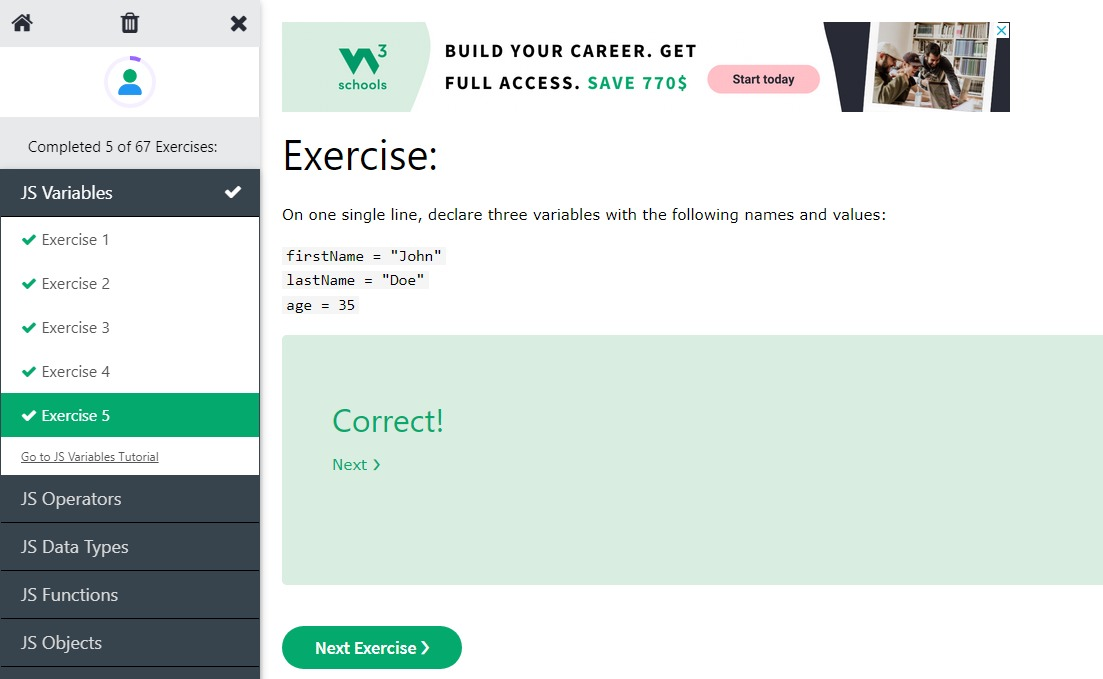
\includegraphics[width=0.9\textwidth,keepaspectratio]{JS VARIABLES.jpeg}

            \newline \newline \newline
            \newline \newline \newline
            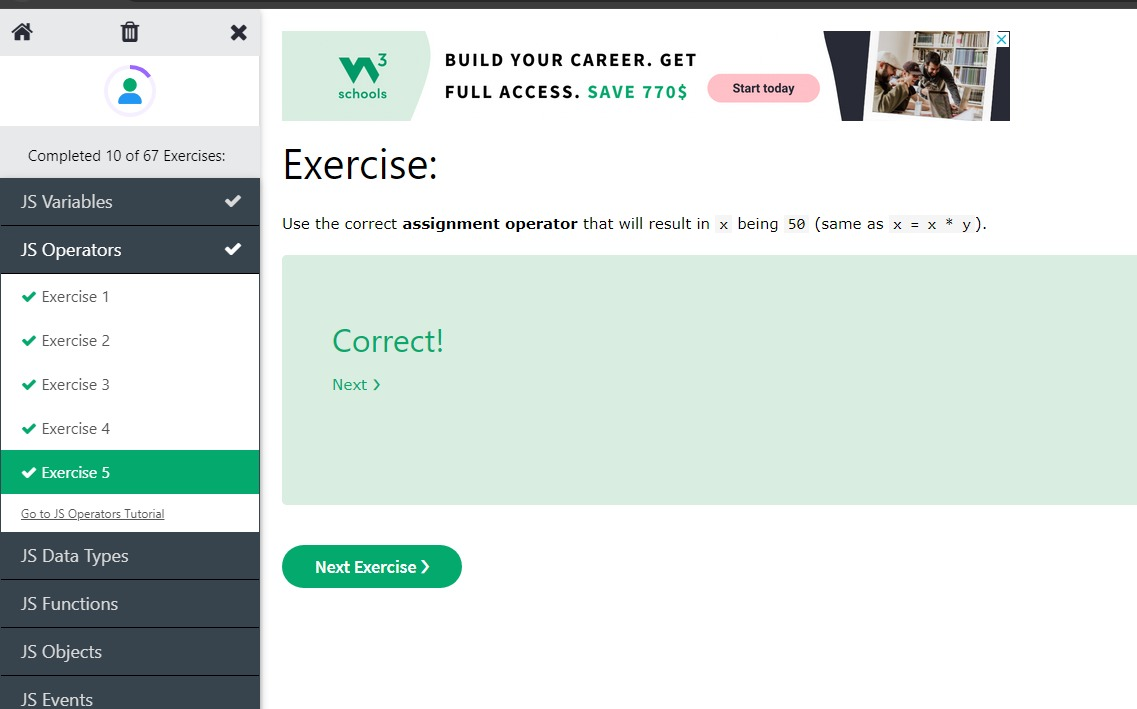
\includegraphics[width=0.9\textwidth,keepaspectratio]{JS OPERATORS.jpeg}

            \newline \newline \newline
            \newline \newline \newline
            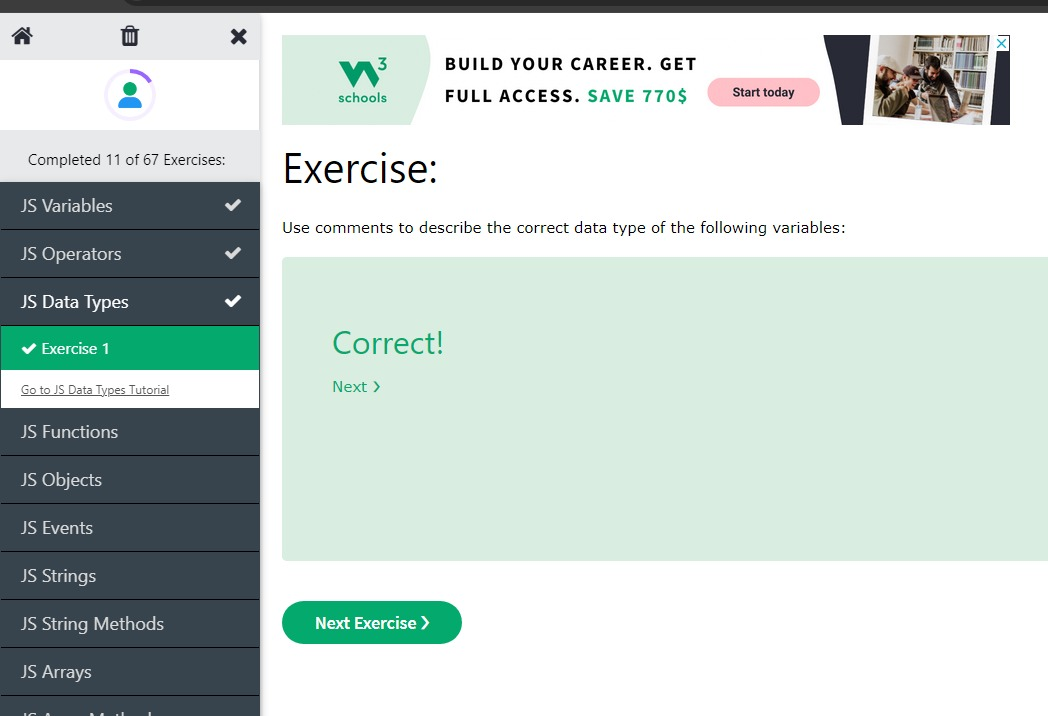
\includegraphics[width=0.9\textwidth,keepaspectratio]{JS DATA TYPES.jpeg}

            \newline \newline \newline
            \newline \newline \newline
            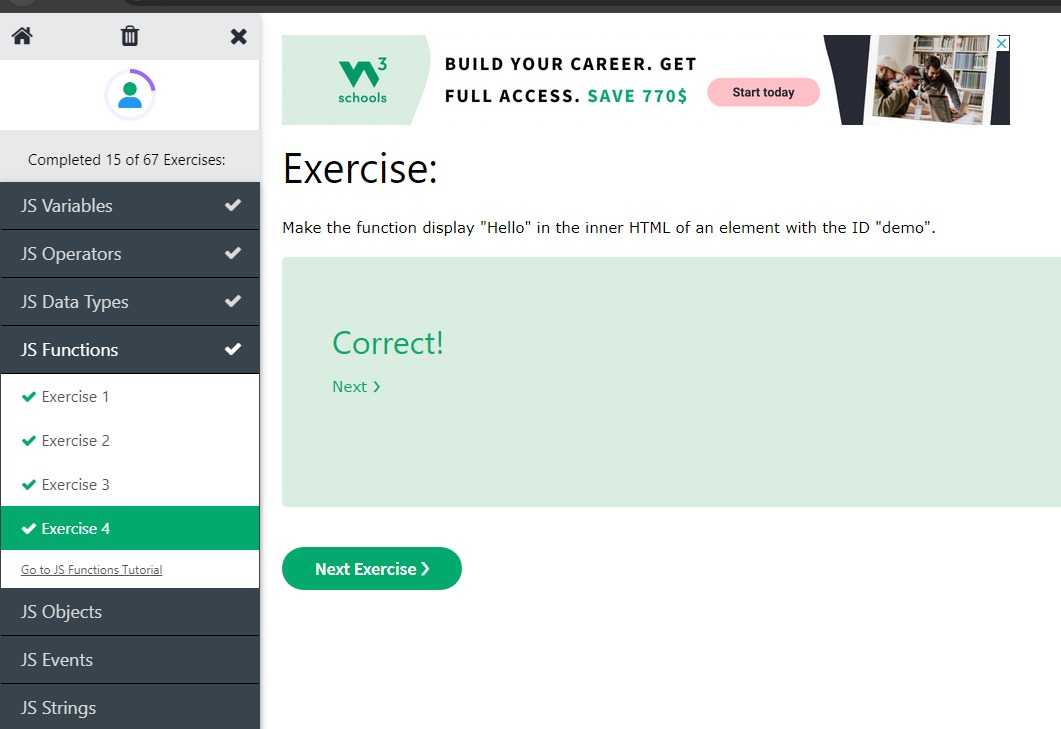
\includegraphics[width=0.9\textwidth,keepaspectratio]{JS FUNCTIONS.jpeg}

            \newline \newline \newline
            \newline \newline \newline
            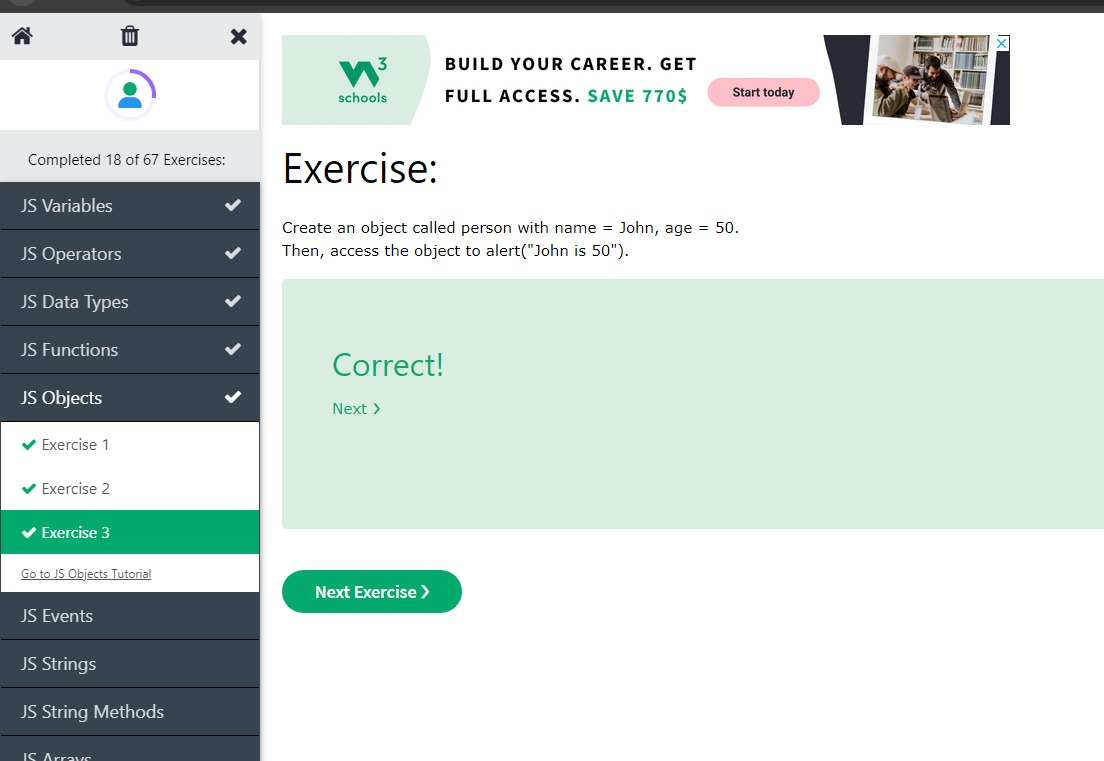
\includegraphics[width=0.9\textwidth,keepaspectratio]{JS OBJECTS.jpeg}

            \newline \newline \newline
            \newline \newline \newline
            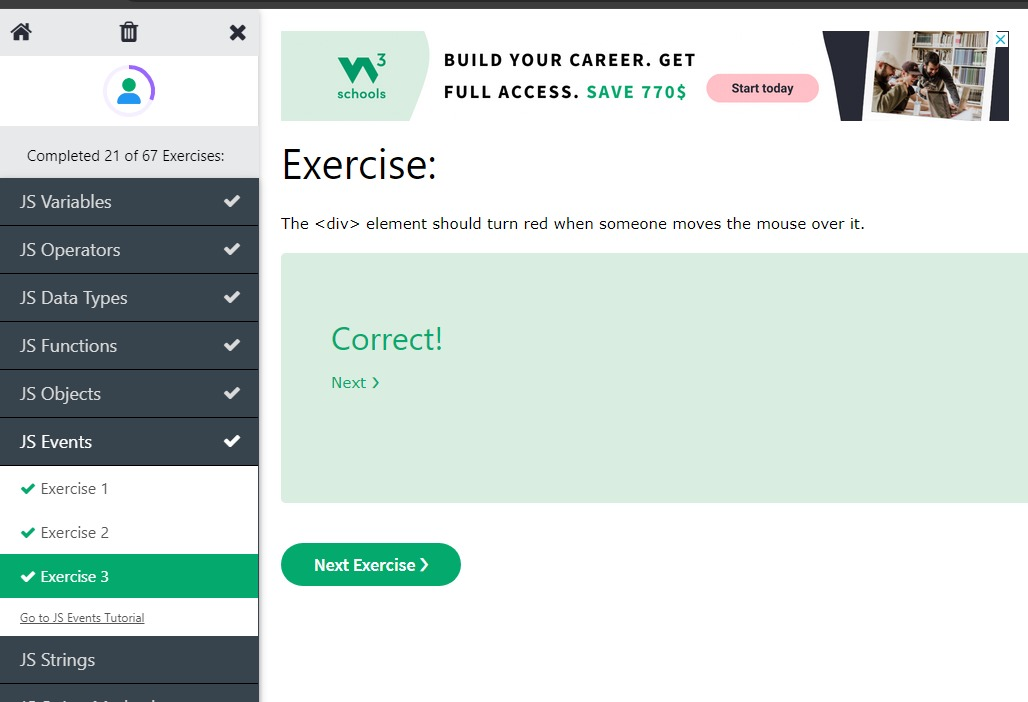
\includegraphics[width=0.9\textwidth,keepaspectratio]{JS EVENTS.jpeg}

            \newline \newline \newline
            \newline \newline \newline
            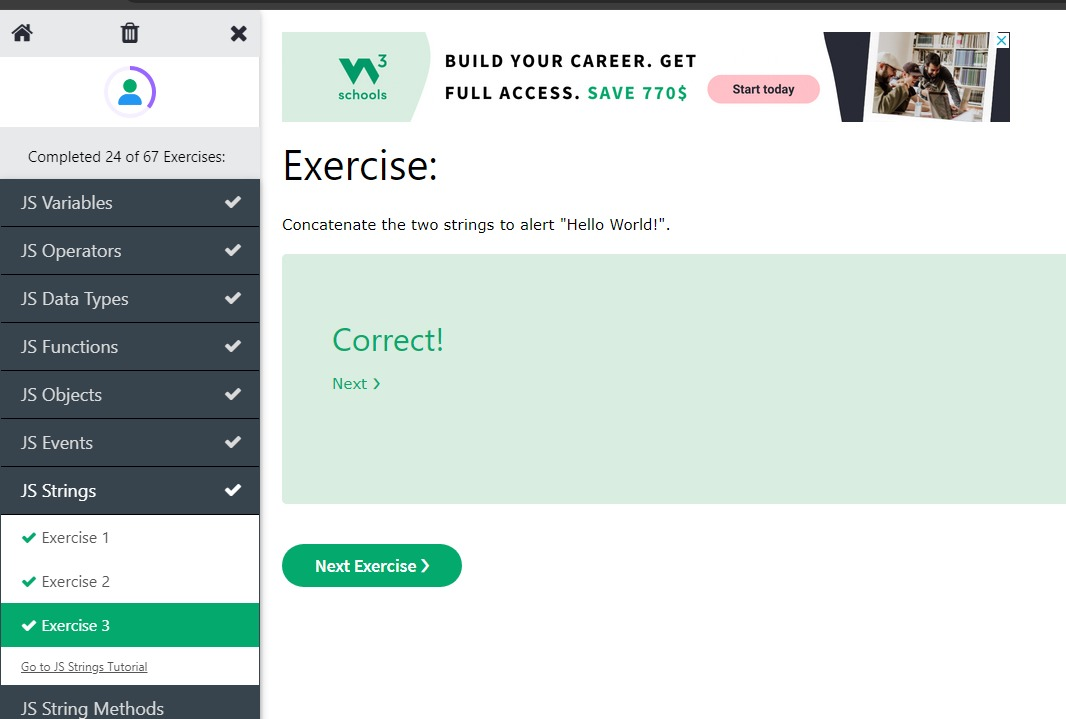
\includegraphics[width=0.9\textwidth,keepaspectratio]{JS STRINGS.jpeg}

            \newline \newline \newline
            \newline \newline \newline
            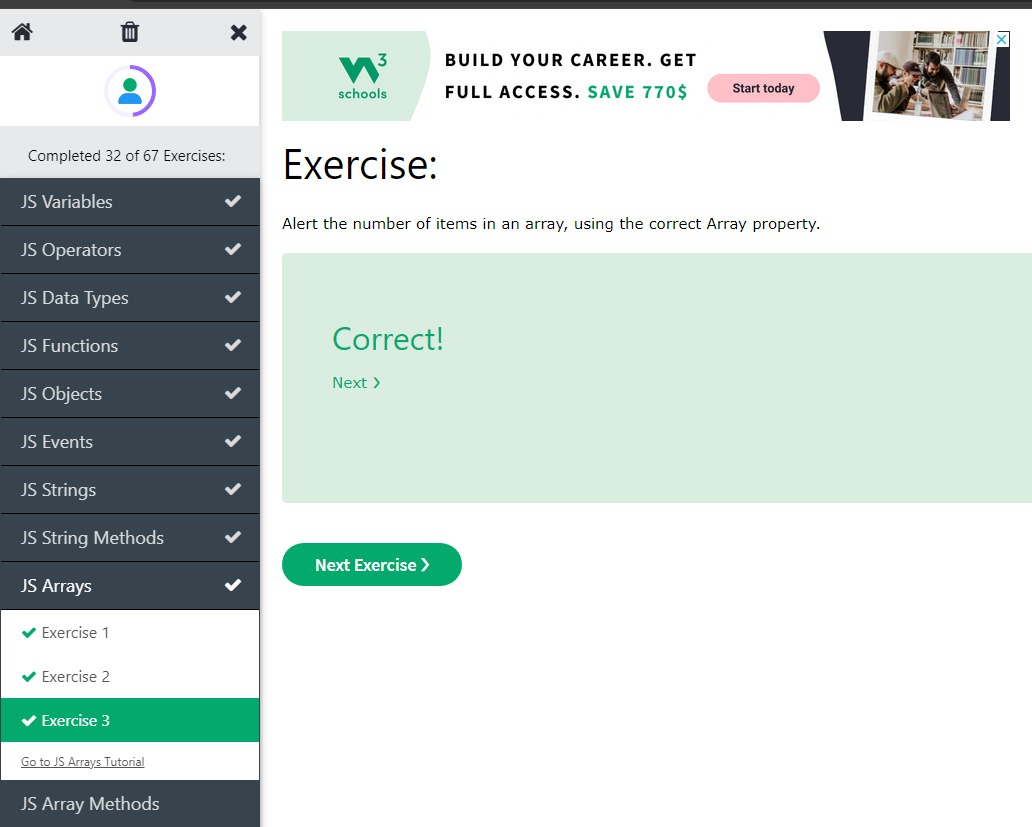
\includegraphics[width=0.9\textwidth,keepaspectratio]{JS ARRAYS.jpeg}

            \newline \newline \newline
            \newline \newline \newline
            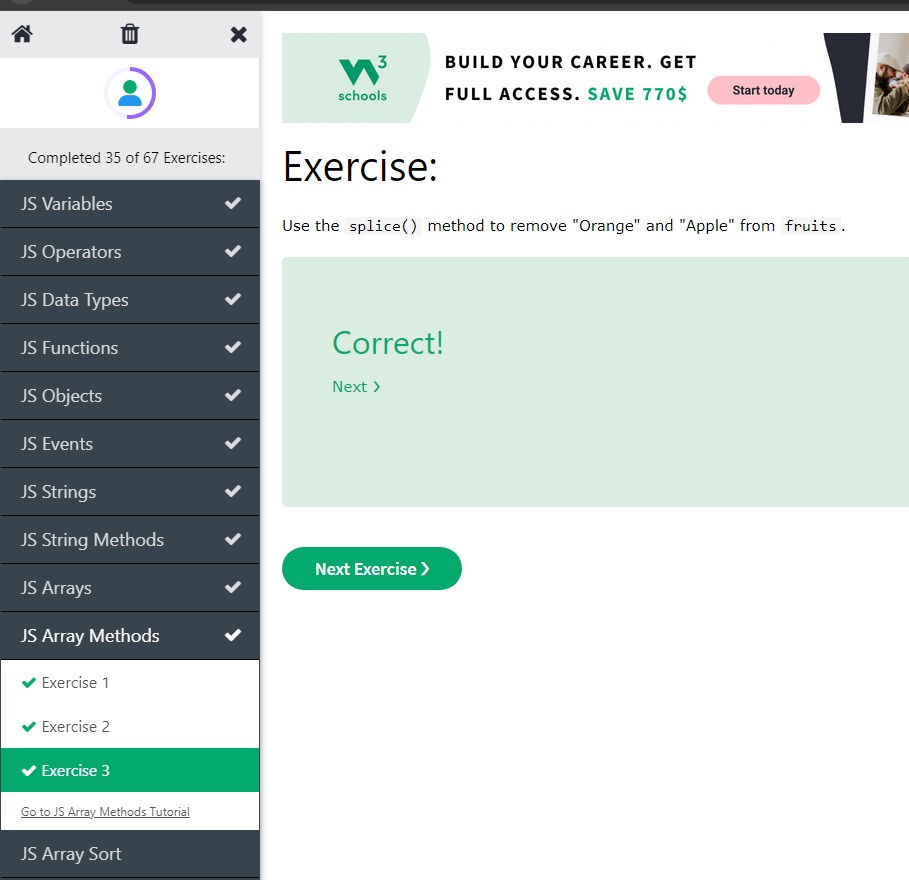
\includegraphics[width=0.9\textwidth,keepaspectratio]{JS ARRAY METHODS.jpeg}

            \newline \newline \newline
            \newline \newline \newline
            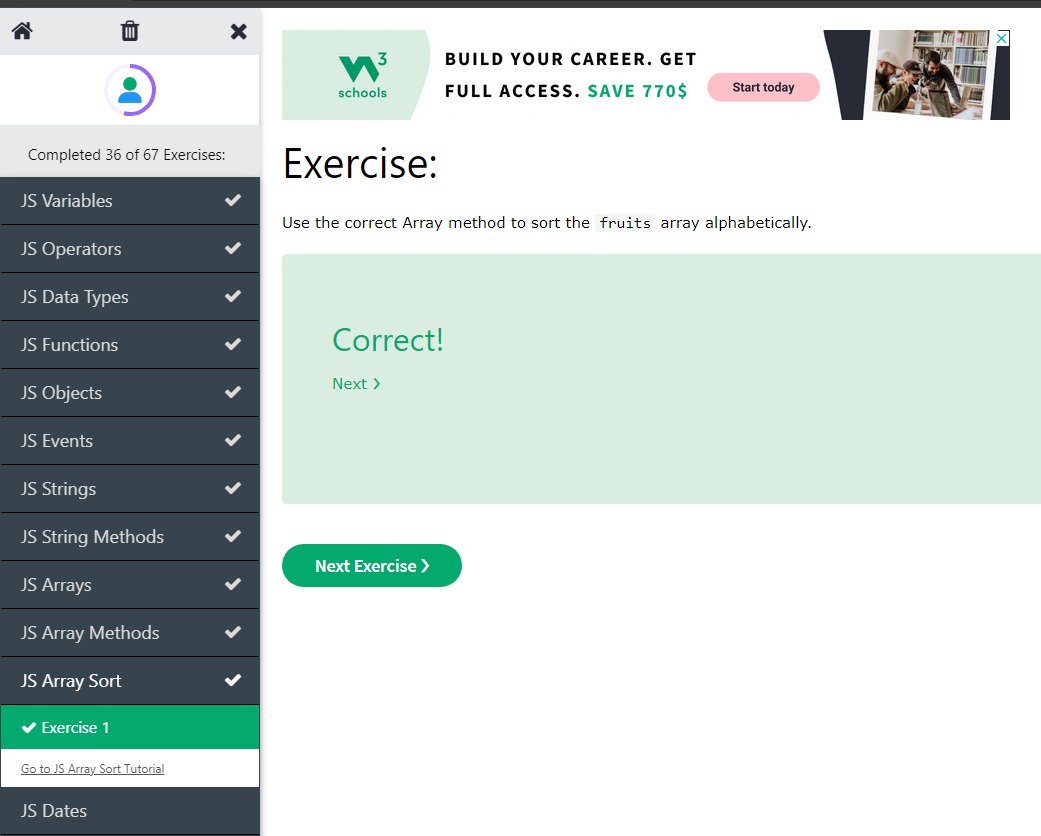
\includegraphics[width=0.9\textwidth,keepaspectratio]{JS ARRAY SORT.jpeg}

            \newline \newline \newline
            \newline \newline \newline
            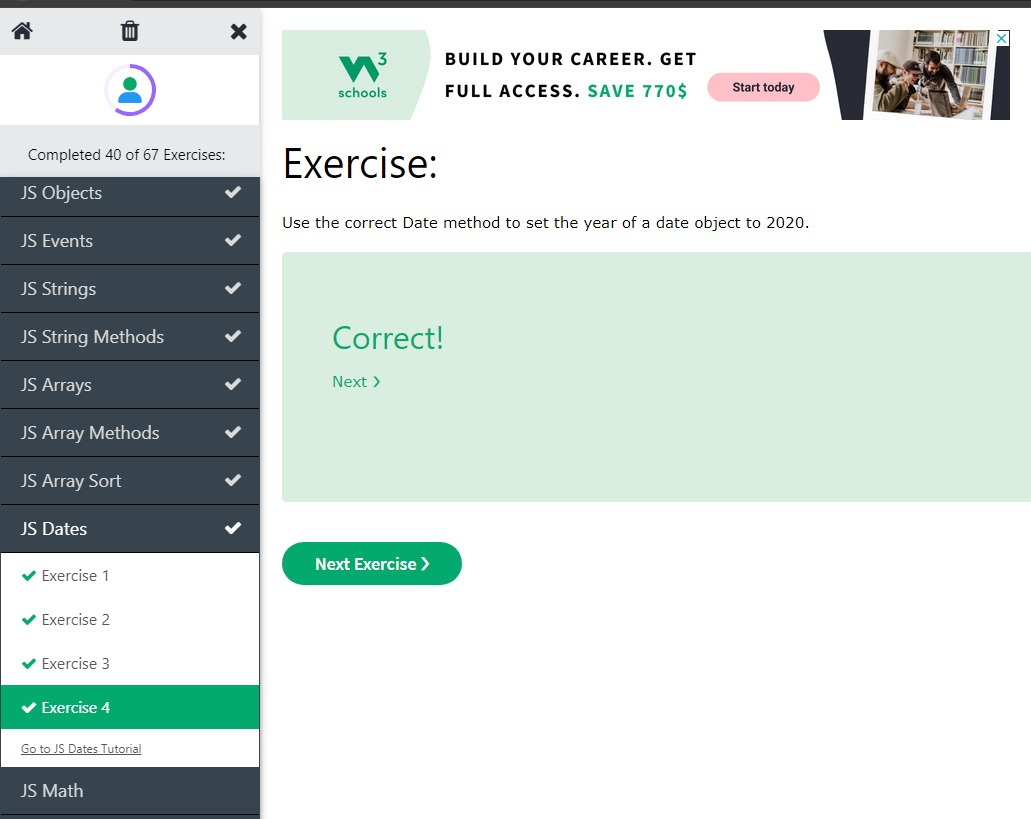
\includegraphics[width=0.9\textwidth,keepaspectratio]{JS DATES.jpeg}

            \newline \newline \newline
            \newline \newline \newline
            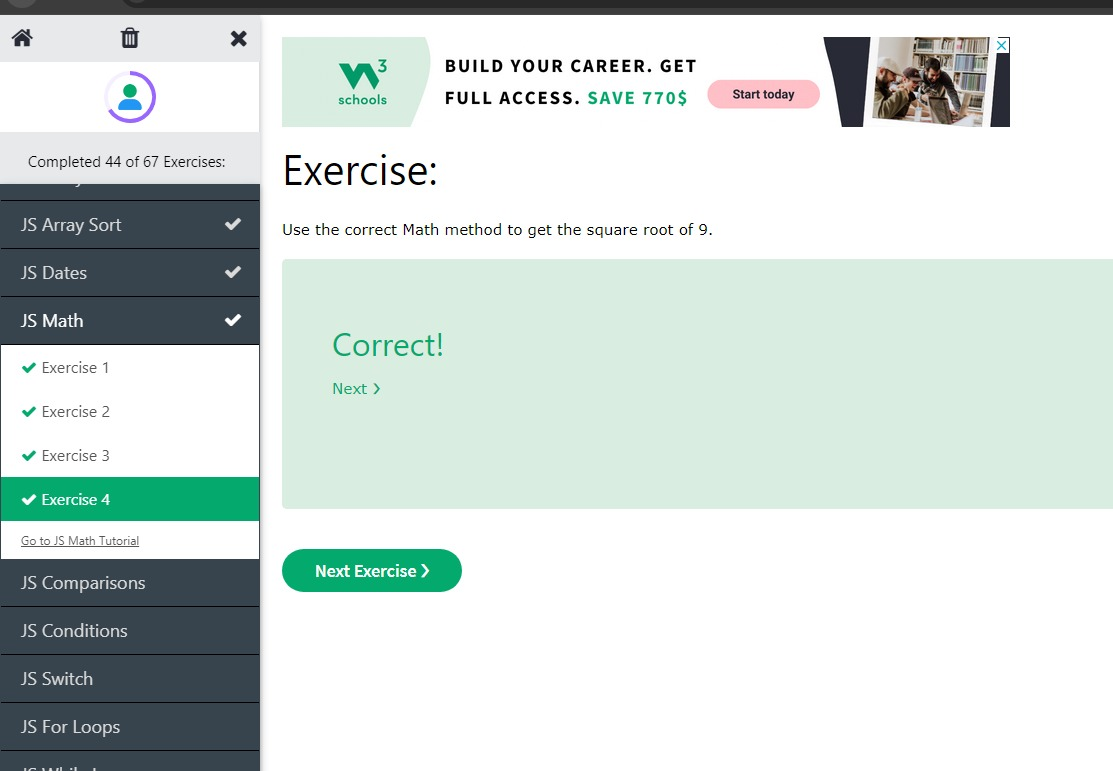
\includegraphics[width=0.9\textwidth,keepaspectratio]{JS MATH.jpeg}

            \newline \newline \newline
            \newline \newline \newline
            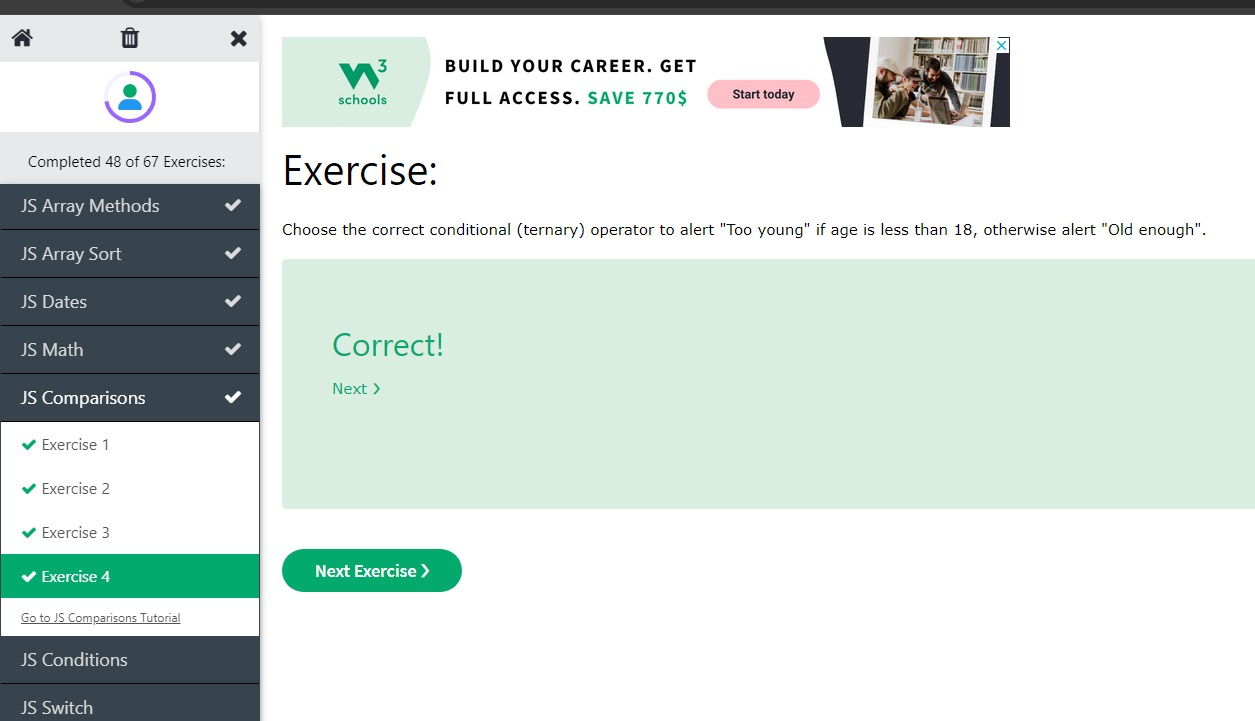
\includegraphics[width=0.9\textwidth,keepaspectratio]{JS COMPARIONS.jpeg}

            \newline \newline \newline
            \newline \newline \newline
            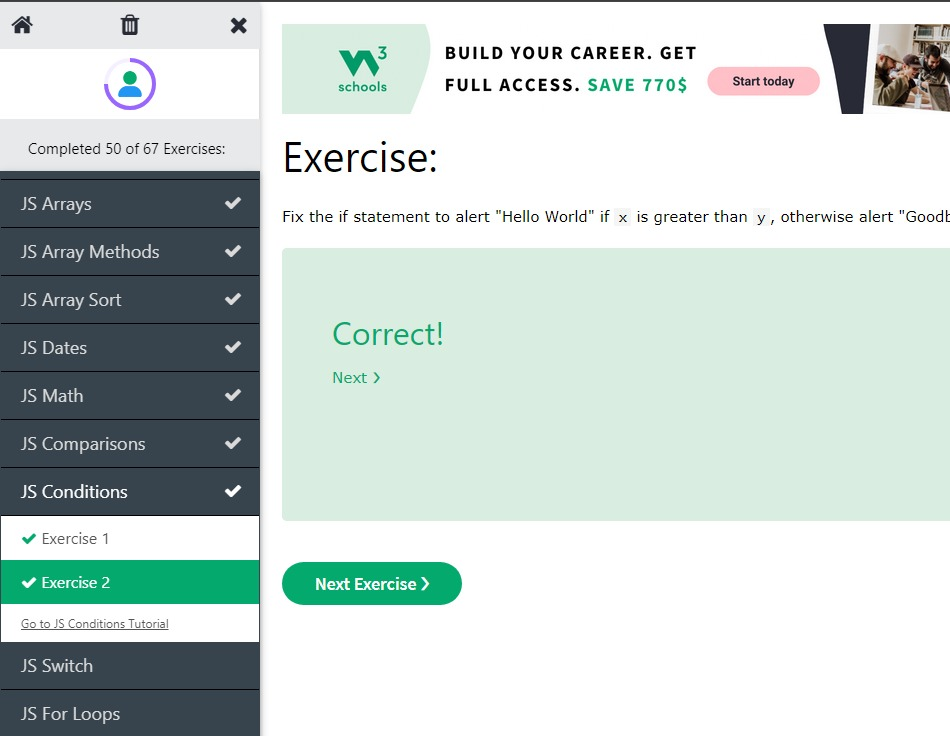
\includegraphics[width=0.9\textwidth,keepaspectratio]{JS CONDITIONS.jpeg}

            \newline \newline \newline
            \newline \newline \newline
            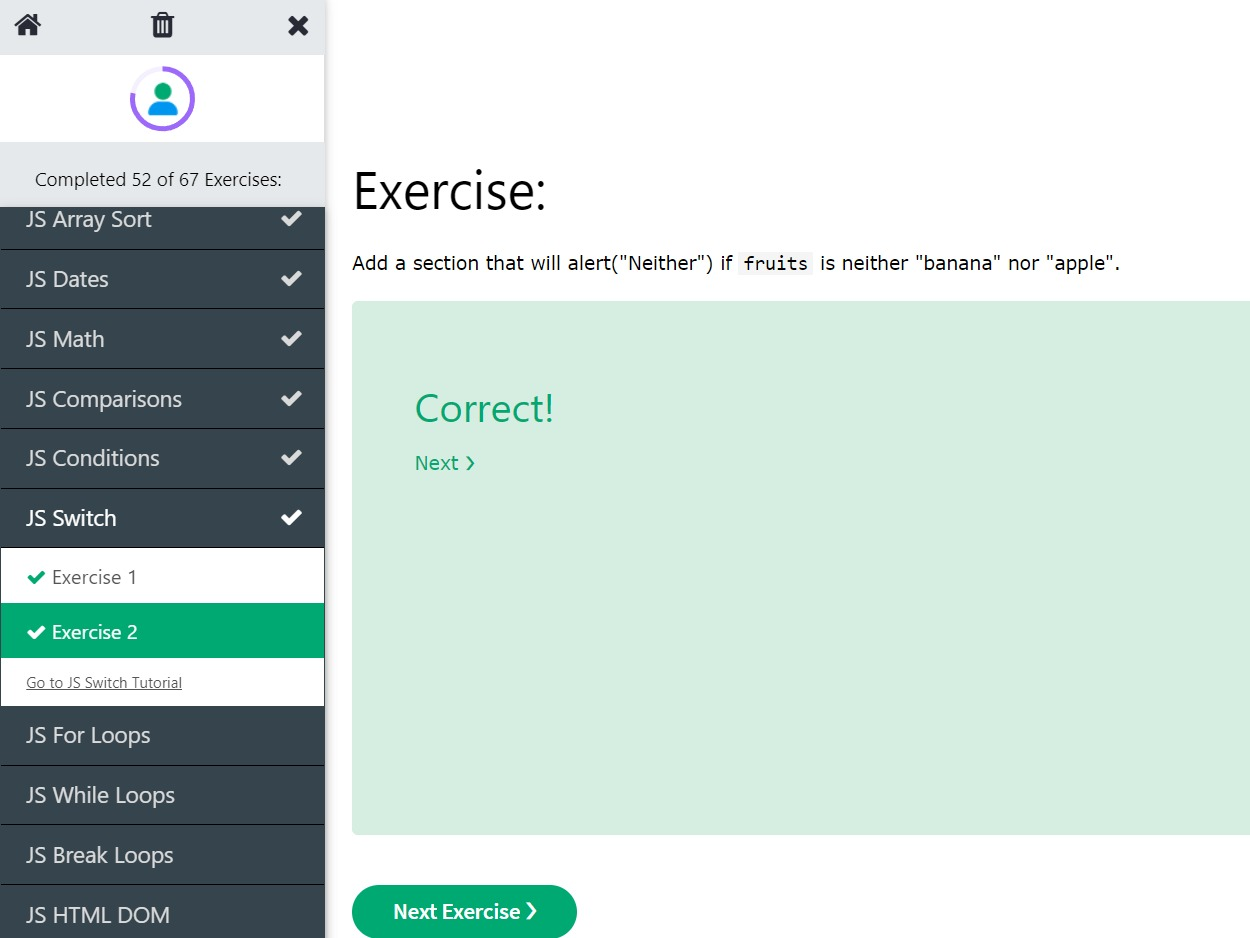
\includegraphics[width=0.9\textwidth,keepaspectratio]{JS SWITCH.jpeg}

            \newline \newline \newline
            \newline \newline \newline
            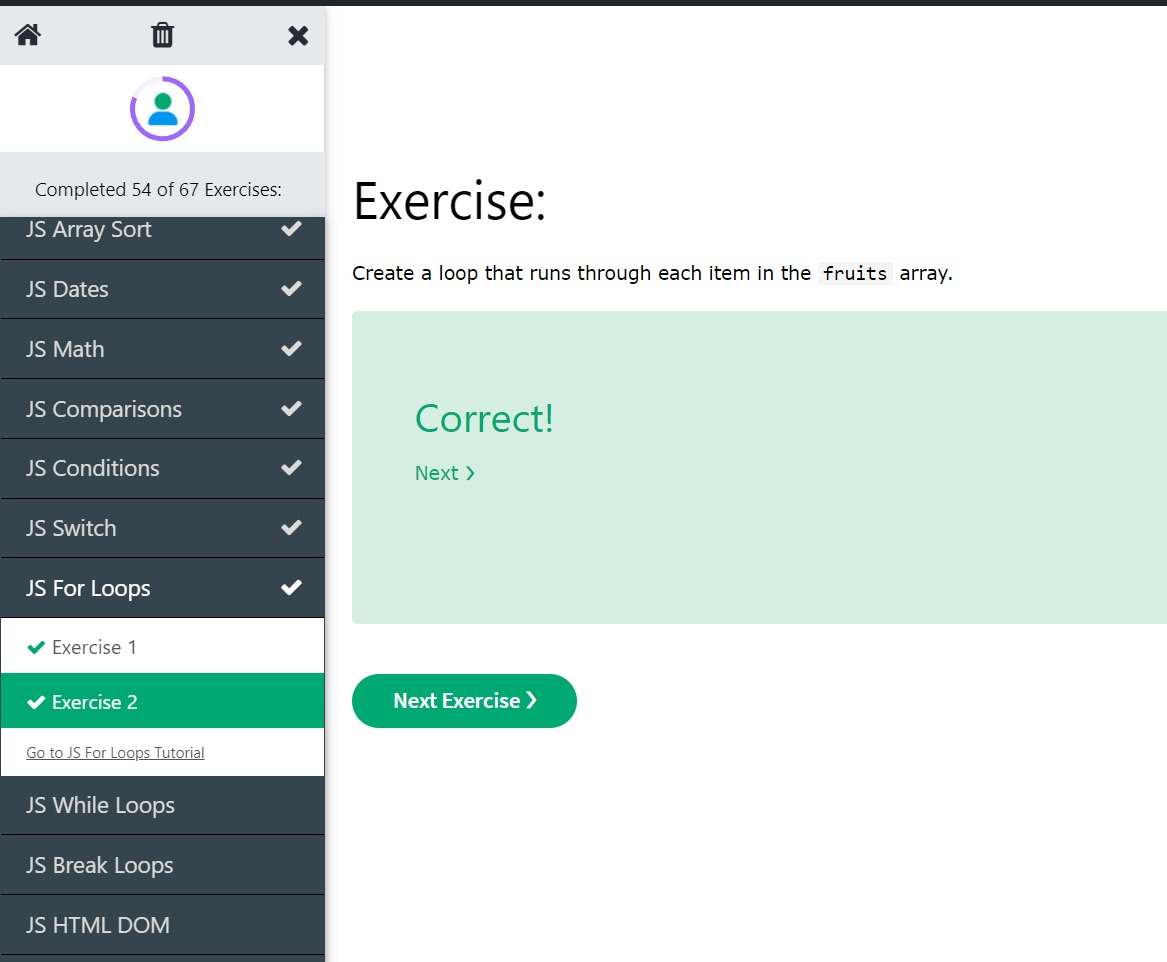
\includegraphics[width=0.9\textwidth,keepaspectratio]{JS FOR LOOPS.jpeg}

            \newline \newline \newline
            \newline \newline \newline
            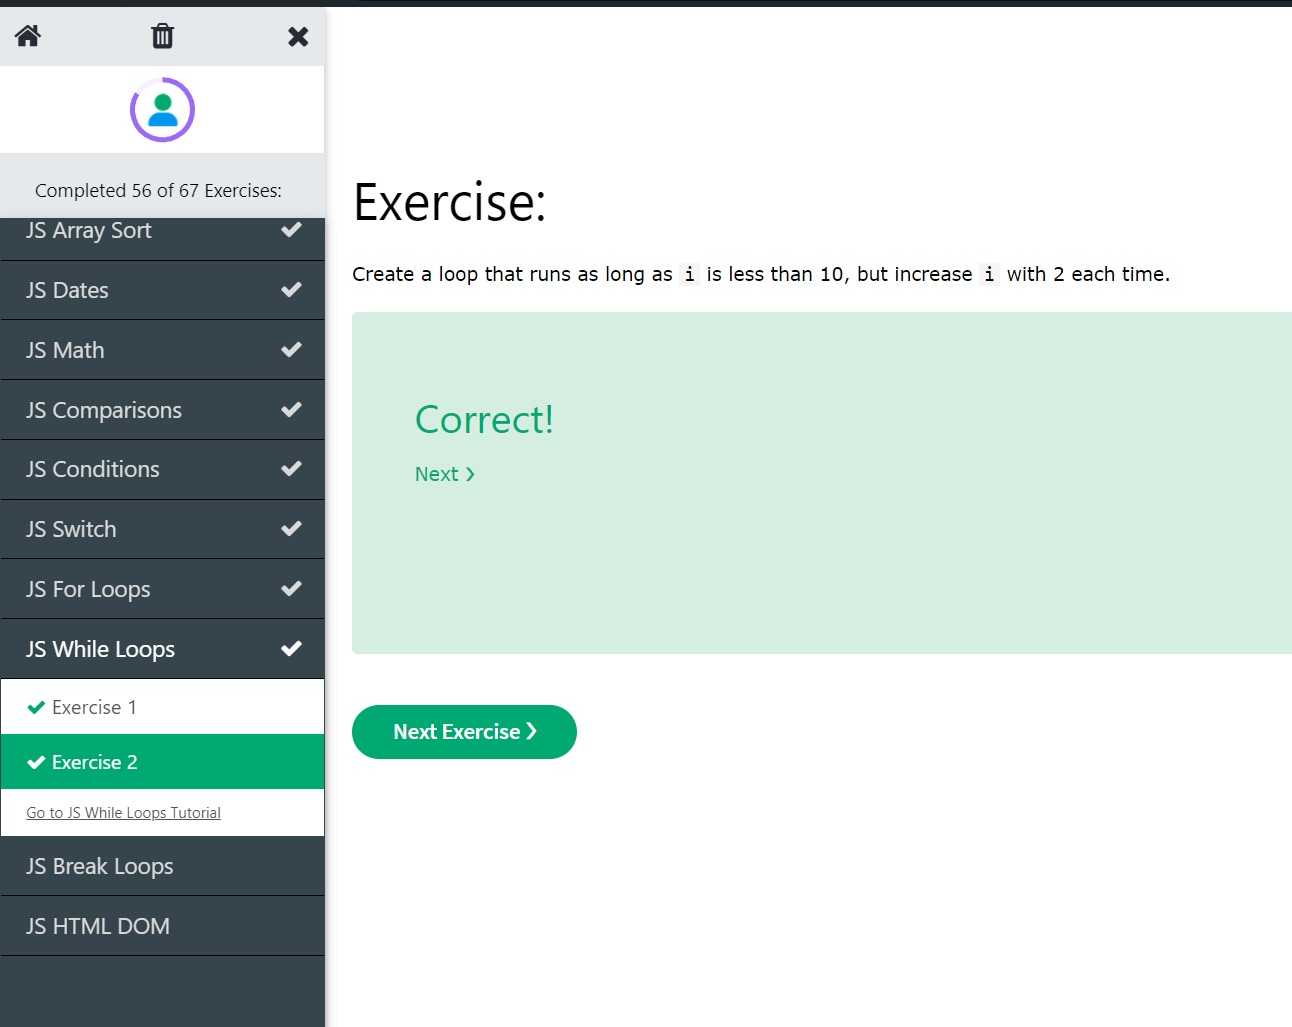
\includegraphics[width=0.9\textwidth,keepaspectratio]{JS WHILE LOOPS.jpeg}

            \newline \newline \newline
            \newline \newline \newline
            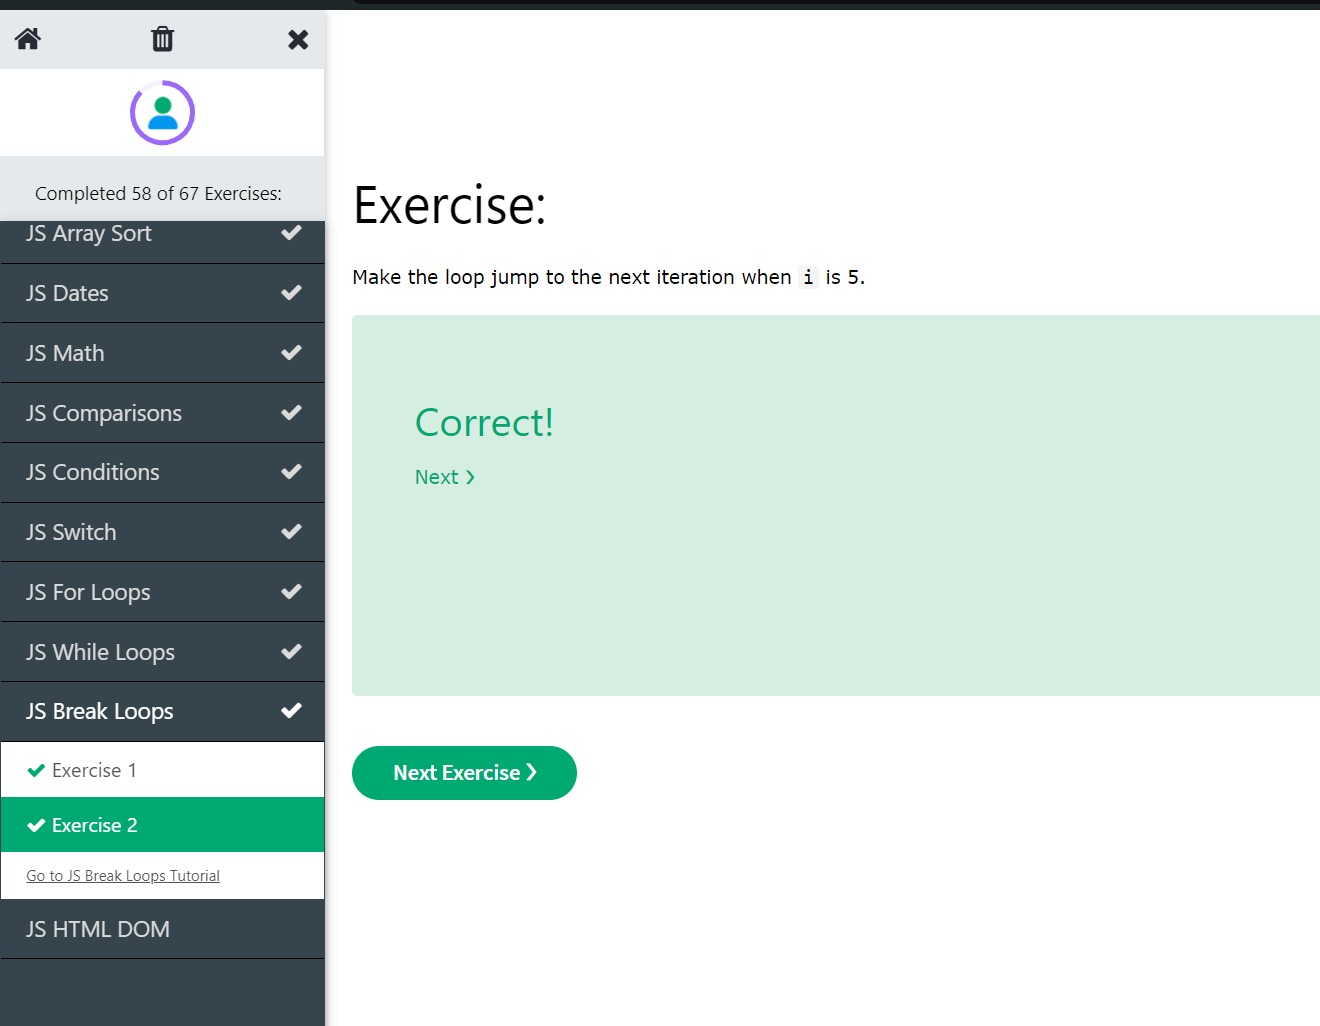
\includegraphics[width=0.9\textwidth,keepaspectratio]{JS BREAK LOOPS.jpeg}

            \newline \newline \newline
            \newline \newline \newline
            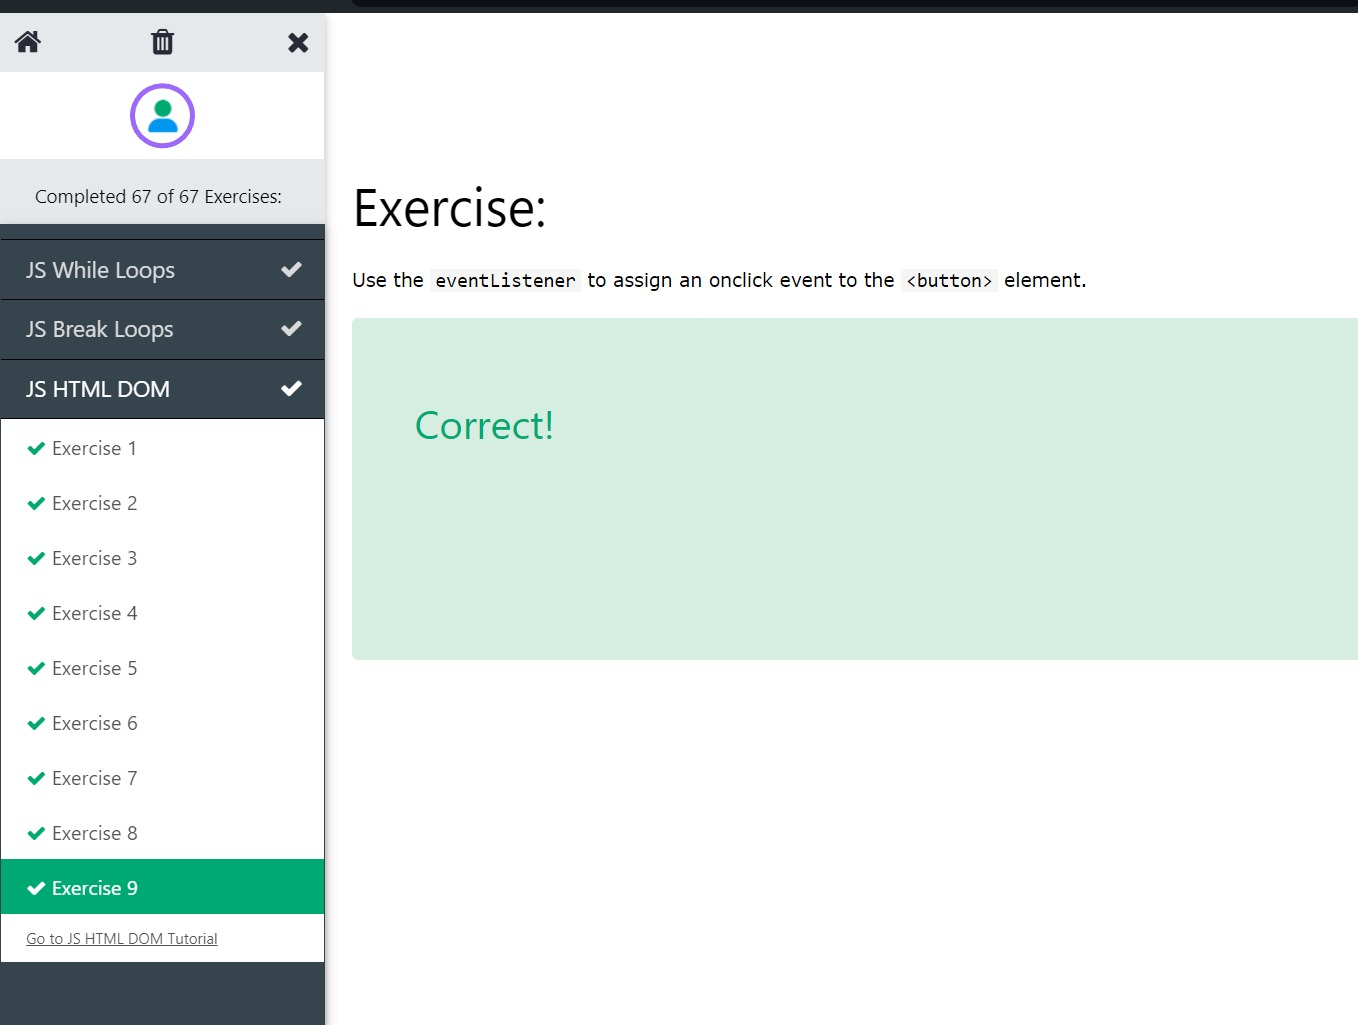
\includegraphics[width= 0.9\textwidth,keepaspectratio]{JS HTML DOM.jpeg}
            
	\end{itemize}	
    \clearpage

	\section{\textcolor{red}{Rúbricas}}
	
	\subsection{\textcolor{red}{Entregable Informe}}
	\begin{table}[H]
		\caption{Tipo de Informe}
		\setlength{\tabcolsep}{0.5em} % for the horizontal padding
		{\renewcommand{\arraystretch}{1.5}% for the vertical padding
		\begin{tabular}{|p{3cm}|p{12cm}|}
			\hline
			\multicolumn{2}{|c|}{\textbf{\textcolor{red}{Informe}}}  \\
			\hline 
			\textbf{\textcolor{red}{Latex}} & \textcolor{blue}{El informe está en formato PDF desde Latex,  con un formato limpio (buena presentación) y facil de leer.}   \\ 
			\hline 
			
			
		\end{tabular}
	}
	\end{table}
	

	
	\subsection{\textcolor{red}{Rúbrica para el contenido del Informe y demostración}}
	\begin{itemize}			
		\item El alumno debe marcar o dejar en blanco en celdas de la columna \textbf{Checklist} si cumplio con el ítem correspondiente.
		\item Si un alumno supera la fecha de entrega,  su calificación será sobre la nota mínima aprobada, siempre y cuando cumpla con todos lo items.
		\item El alumno debe autocalificarse en la columna \textbf{Estudiante} de acuerdo a la siguiente tabla:
	
		\begin{table}[ht]
			\caption{Niveles de desempeño}
			\begin{center}
			\begin{tabular}{ccccc}
    			\hline
    			 & \multicolumn{4}{c}{Nivel}\\
    			\cline{1-5}
    			\textbf{Puntos} & Insatisfactorio 25\%& En Proceso 50\% & Satisfactorio 75\% & Sobresaliente 100\%\\
    			\textbf{2.0}&0.5&1.0&1.5&2.0\\
    			\textbf{4.0}&1.0&2.0&3.0&4.0\\
    		\hline
			\end{tabular}
		\end{center}
	\end{table}	
	
	\end{itemize}
	
	\begin{table}[H]
		\caption{Rúbrica para contenido del Informe y demostración}
		\setlength{\tabcolsep}{0.5em} % for the horizontal padding
		{\renewcommand{\arraystretch}{1.5}% for the vertical padding
		%\begin{center}
		\begin{tabular}{|p{2.7cm}|p{7cm}|x{1.3cm}|p{1.2cm}|p{1.5cm}|p{1.1cm}|}
			\hline
    		\multicolumn{2}{|c|}{Contenido y demostración} & Puntos & Checklist & Estudiante & Profesor\\
			\hline
			\textbf{1. GitHub} & Hay enlace URL activo del directorio para el  laboratorio hacia su repositorio GitHub con código fuente terminado y fácil de revisar. &2 &X &2 & \\ 
			\hline
			\textbf{2. Commits} &  Hay capturas de pantalla de los commits más importantes con sus explicaciones detalladas. (El profesor puede preguntar para refrendar calificación). &4 &X &2 &  \\ 
			\hline 
			\textbf{3. Código fuente} &  Hay porciones de código fuente importantes con numeración y explicaciones detalladas de sus funciones. &2 &X &2 & \\ 
			\hline 
			\textbf{4. Ejecución} & Se incluyen ejecuciones/pruebas del código fuente  explicadas gradualmente. &2 &X &1 & \\ 
			\hline			
			\textbf{5. Pregunta} & Se responde con completitud a la pregunta formulada en la tarea.  (El profesor puede preguntar para refrendar calificación).  &2 &X &2 & \\ 
			\hline	
			\textbf{6. Fechas} & Las fechas de modificación del código fuente estan dentro de los plazos de fecha de entrega establecidos. &2 &X &2 & \\ 
			\hline 
			\textbf{7. Ortografía} & El documento no muestra errores ortográficos. &2 &X &2 & \\ 
			\hline 
			\textbf{8. Madurez} & El Informe muestra de manera general una evolución de la madurez del código fuente,  explicaciones puntuales pero precisas y un acabado impecable.   (El profesor puede preguntar para refrendar calificación).  &4 &X &4 & \\ 
			\hline
			\multicolumn{2}{|c|}{\textbf{Total}} &20 & &17 & \\ 
			\hline
		\end{tabular}
		%\end{center}
		%\label{tab:multicol}
		}
	\end{table}
	
\clearpage
	
	
%\clearpage
%\bibliographystyle{apalike}
%\bibliographystyle{IEEEtranN}
%\bibliography{bibliography}
			
\end{document}
